\documentclass[a4paper]{article}

\usepackage{a4wide}
\usepackage{amssymb}
\usepackage{xcolor}
\usepackage{comment}
\usepackage{graphicx}
\usepackage[dutch]{babel}

\title{Elektronisch stemmen \\ \large De ethische discussie over elektronisch stemmen in de digitale samenleving.}
\author{
Mick van Gelderen \\ 4091566 \and 
Mick de Lange \\ 1534068 \and
Salim Salmi \\ 4089715
}


\newcommand{\TODO}[1]{{\color{red}\textbf{TODO: #1}}}

\usepackage{amsmath}
\begin{document}

\thispagestyle{plain}
\maketitle

\hfill \\ \\ \\ \\ \\ \\ \\ \\ \\ \\
\begin{figure}[htp]
\centering
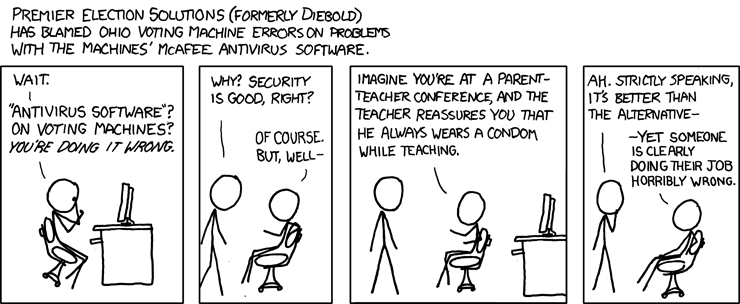
\includegraphics[width=\textwidth]{media/voting_machines.png}
\label{fig:voting-machines}
\begin{comment}
Randall Munroe, (2013), Voting Machines [ONLINE]. Available at: http://imgs.xkcd.com/comics/voting_machines.png [Accessed 15 March 13].
\end{comment}
\end{figure}

\newpage

\thispagestyle{plain}

\section*{Voorwoord}
Dit artikel is geschreven door 3 studenten Technische Informatica aan de Technische Universiteit Delft voor het vak `informatietechnologie en waarden'.
Het belicht een ethische kwestie van verschillende standpunten aangesterkt met literatuur uit het vakgebied en de filosofie. 

\section*{Samenvatting}

\newpage

\thispagestyle{plain}
\renewcommand{\contentsname}{Inhoud} 
\tableofcontents

\newpage

\section{Inleiding}

In de afgelopen jaren is er in Nederland veel te doen geweest rondom elektronisch stemmen.
Zo zijn er een aantal proeven geweest, met verschillende vormen van elektronisch stemmen.
Er zijn naar aanleiding van een aantal problemen actiegroepen opgericht die zich duidelijk uitspraken tegen elektronisch stemmen.
De overheid heeft uiteindelijk verschillende commissies ingesteld die onderzoek hebben gedaan naar de problemen en naar de benodigdheden om in de toekomst elektronisch stemmen in te voeren.

Er spelen binnen dit onderwerp verschillende technische en morele onderwerpen.
Veel genoemd zijn privacy en veiligheid, maar ook de mogelijkheid om bijvoorbeeld gemakkelijker en sneller de stemmen te tellen.
Er zijn op het gebied van elektronisch stemmen dan ook veel problemen, maar ook voordelen.
Op het moment gebruiken we in Nederland weer het papieren stembiljet, maar er zijn ook landen waar wel elektronisch gestemd kan worden.
Wij willen in dit artikel in gaan op de verschillende aspecten en onderzoeken wat deze problemen en voordelen met zich mee brengen.

Allereerst zullen we hier onze onderzoeksvraag definiëren, dit wordt het uitgangspunt van dit paper en de leidraad van onze uiteindelijke conclusie.
Vervolgens zullen we de gebruikte definitie van elektronisch stemmen bepalen en de verschillende technische en morele aspecten die er spelen belichten.
Aan de hand van deze aspecten zullen we de argumenten voor elektronisch stemmen uiteenzetten.
Daarna zetten we de argumenten tegen elektronisch stemmen op een rijtje.
Uiteindelijk zullen we aan de hand van deze argumenten onze eigen positie in deze ethische discussie bepalen en toelichten hoe en waarom wij tot deze conclusie zijn gekomen.

\subsection{Onderzoeksvraag}

Onze onderzoeksvraag luidt: ``Zouden we over moeten stappen op elektronisch stemmen?''.

Om deze vraag te beantwoorden zullen de verschillende aspecten rondom elektronisch stemmen ter discussie moeten worden gesteld.
Het belichten van deze aspecten en beargumenteren van de pro en con argumenten zal dan uiteindelijk leiden tot een antwoord op deze vraagstelling.

Hierna zullen we eerst verder ingaan op de door ons gebruikte definitie van elektronisch stemmen en de aspecten die daarbij relevant zijn.

\section{Elektronisch stemmen}

Ten eerste zal wat meer inzicht worden gegeven over het elektronische stemmen. 
In dit onderdeel zullen eerst de actoren die een rol spelen worden voorgesteld. 
Daarna worden een aantal technische feiten beschreven zodat het duidelijk is waar elektronisch stemmen over gaat.
Tevens zullen de verschillende morele aspecten omringd het elektronisch stemmen worden beschreven.
Ten slotte zullen de juridische aspecten die bij het elektronische stemmen komen kijken worden besproken.

\subsection{Betrokken partijen}

De twee meest voor de hand liggende partijen bij verkiezingen zijn natuurlijk de politieke partijen en de burgerlijke kiezers. 
Beide hebben echter zeer verschillende belangen en standpunten. 
Andere betrokkenen zijn de fabrikanten van de stemapparatuur en software.
Dit zijn partijen die direct te maken hebben met de uitkomst.
Er zijn daarnaast ook nog specifieke voor en tegenstanders in dit debat.
Een grote tegenstander zijn de mensen van "Wij vertrouwen stemcomputers niet ".
Minister Plasterk is en van de grootste voorstanders van elektronisch stemmen.
 
\subsubsection{Burgelijke kiezers}
De kiezer is de grootste van alle betrokken partijen.
Voor de kiezer is het natuurlijk belangrijk dat hun stem correct wordt genoteerd en opgeslagen. 
Betrouwbaarheid is voor de burgers dus een belangrijk aspect.
De burger wil tevens niet dat hun privacy op het spel komt te staan.
 
\subsubsection{Politieke partijen}
Net zo zeer als burgers hun stem willen waarborgen, willen de politieke partijen dat hun stem niet zomaar door een fout naar een andere partij gaat.
Ook fraude zal voor de politieke partijen een belangrijke rol spelen. 
Een elektronisch systeem waar makkelijk fraude op gepleegd kan worden zal natuurlijk niet zomaar geaccepteerd worden.

\subsubsection{Fabrikanten van de stemapparatuur}
De voornaamste leverancier van stemapparatuur in het verleden was een bedrijf genaamd Nedap.
Nedap levert bijna 90 procent van alle stemcomputers in Nederland.
Toen in 2007 het elektronische stemmen weer werd vervangen door potlood en papier heeft dit voor het bedrijf natuurlijk grote gevolgen gehad.
Daarentegen werd een zekere kwaliteiten waarborging verwacht waar niet aan gehouden was.
Om een actor in dit debat te kunnen blijven zullen de fabrikanten van stemapparatuur en software in moeten kunnen stemmen met de wensen van andere betrokkenen.

\subsubsection{Wij vertrouwen stemcomputers niet}
In 2006 heeft deze groep een website opgericht tegen het gebruik van stemcomputers. 
Zij kwamen toen met het punt dat stemcomputers de verkiezingen voor de burger oncontroleerbaar maken.
Ook vonden zij dat de regelgeving en de techniek van de stemcomputers te kort schoten.

\subsubsection{Minister Plasterk}
Minister van Binnenlandse Zaken heeft aangegeven dat hij pleit om weer te kijken naar het gebruik van stemcomputers.
Stemmen met het rode potlood is niet meer van deze tijd zegt hij. 
Volgens Plasterk is de techniek al veel vooruitgegaan sinds 2007 toen het gebruik van stemcomputers werd verboden vanwege fraude mogelijkheden.


\subsection{Technische feiten}

Als men het over elektronisch stemmen heeft dan wordt bedoelt het op een over ander manier vastleggen van jouw stem vast te leggen op een digitaal systeem.
Hier is echter nog niet alles mee gezegd, want dit kan op een groot aantal verschillende manieren gebeuren en elk van deze technieken heeft een aantal gevolgen voor de actoren. 

\subsubsection{Stemmen in het stemlokaal}
De huidige manier van stemmen betreft het invullen van de keuze op een voorgedrukt papieren stembiljet. 
Echter kan er zelfs op dit niveau al techniek aan te pas komen door middel van het scannen van de keuze gemaakt op het stembiljet en deze elektronisch vast te leggen.
Een andere mogelijkheid van elektronisch stemmen is het gebruik van een elektronisch stemapparaat met daarnaast een papieren stembiljet voor controle.
Ten slotte kan ook gebruikt gemaakt worden van een stemprinter. 
Hierbij maakt de kiezer elektronisch zijn stem die vervolgens wordt uitgeprint en elektronisch wordt geteld.
Dit zijn allemaal manieren om elektronisch stemmen te combineren met het papieren stem systeem.
Het voornaamste doel van het implementeren van technologie is hier het vergemakkelijken van de stemmentelling.
Op dit moment worden al naar deze oplossingen gekeken en mee ge{\"e}xperimeerd.

\subsubsection{Stemmen over het internet}
Tot nu zijn verschillende alternatieven beschreven voor het stemmen in het stemlokaal, waar stemmen priv{\'e} wordt gedaan. 
Maar hoe zit het met stemmen vanuit huis?
Door de opkomst van het internet is de mogelijkheid ontstaan om via het internet te stemmen.
Bij dit gemak komen ook problemen kijken, zoals veiligheid en fraude. 
Het stemmen over het internet heeft echter een groot fundamenteel probleem waardoor er van wordt afgezien.
Er is namelijk geen manier om besloten stemmen te kunnen waarborgen.
Potenti{\"e}le gevolgen kunnen zijn dat bijvoorbeeld druk kan worden uitgeoefend op de kiezer waardoor de kiezer niet meer voor zichzelf stemt.

\subsection{Morele aspecten}
Om te bepalen welke morele aspecten er spelen rondom elektronisch stemmen, zullen we eerst moeten kijken naar de geldende normen en waarden rondom het uitbrengen van een stem.
In de huidige vorm van stemmen, met papieren biljetten, zijn een aantal waarden die een belangrijke rol spelen.
Niet al deze waarden hebben altijd een dergelijke rol gehad bij eerdere stemmethoden.
Bij het invoeren komen van elektronisch stemmen zijn er ook nog andere waarden die een rol gaan spelen, deze komen hier ook aan bod.

\subsubsection{Privacy}
In het huidige kiessysteem is het erg belangrijk dat we onze daadwerkelijke stem voor ons zelf houden.
Ondanks dat iedereen kan vertellen wat hij heeft gestemd, hoeft dit niet de waarheid te zijn en kan iedereen de stem uitbrengen die hij zelf wil.
Deze norm is ontstaan uit de angst voor afpersing of bedreiging, waardoor een kiezer gedwongen kan worden anders te stemmen dan zijn eigen voorkeur.
Omdat dit als een zodanig belangrijk punt wordt gezien is deze norm ook opgenomen in de wetgeving, hierover meer in het onderdeel `Juridische aspecten'.

Overigens speelde privacy niet altijd een dergelijke rol bij het uitbrengen van stemmen.
Zo werd er vroeger ook wel mondeling gestemd, waarbij een persoon fysiek in een publieke ruimte zijn stem uitsprak.
Hierbij was het dus mogelijk om precies te zien wie wat stemde, iets wat in die periode juist als een belangrijke waarde werd gezien.

\subsubsection{Vrijheid}
Vrijheid is enigszins gekoppeld aan de voorgaande waarde, het gaat hier namelijk om de vrijheid om zelf te bepalen welke partij jouw stem verdient.
Deze waarde staat ook weer in verband met het probleem van afpersing of bedreiging.
Vrijheid zou gezien kunnen worden als de onderliggende waarde voor de norm over privacy in het uitbrengen van een stem.
Om een democratisch systeem te laten werken vinden mensen het van belang dat ieder persoon kan stemmen op de persoon of partij van zijn eigen voorkeur, zonder dat invloeden van buiten af effect hebben op deze keuze.

Ook zijn er natuurlijk andere factoren die invloed kunnen uitoefenen op de stemvoorkeur van een persoon, zoals media en campagne voering, of bijvoorbeeld groepsdruk.
Deze factoren spelen weliswaar een rol in de keuzevrijheid van het individu, maar zijn even belangrijk bij zowel het huidige papieren stemmen als elektronisch stemmen.
Hier zullen we dan ook niet al te ver op in gaan in dit paper.

\subsubsection{Eerlijkheid}
Bij verkiezingen is eerlijkheid ook een belangrijke waarde, hierbij gaat het dan met name over de eerlijkheid van het proces van de stemmen telling.
Stemmen tellen gebeurt in de huidige papieren vorm, met de hand.
Deze mensen die de telling uitvoeren controleren elkaar, om grote fouten te voorkomen.
In verkiezingen vinden we het belangrijk dat elke partij of kiespersoon de stemmen krijgt die ook daadwerkelijk zijn uitgebracht op die persoon of partij.

Eerlijkheid is heel duidelijk een waarde die in alle vormen van stemmen terug komt.
Zowel in oudere varianten als in elektronisch stemmen speelt dit een rol.
Immers om een juiste verkiezingsuitslag te garanderen is een eerlijke telling van groot belang.

Door middel van openheid in het proces van stemmen tellen probeert men deze eerlijkheid te garanderen.
Het proces moet een open karakter hebben, zodat elke burger begrijpt en ziet hoe de stemmen worden geteld.
Dit begrip en inzicht is voor de burger die zijn stem uitbrengt essentieel om vertrouwen te hebben in het proces.

\subsection{Juridische aspecten}

\subsubsection{Stemgeheim}
Deze wetgeving betekent in de praktijk dus dat het niet is toegestaan om samen met iemand anders een stem uit te brengen.
Vandaar ook de verplichting van maximaal {\'e}{\'e}n persoon in een stemhokje.

Het stemgeheim speelt ook een belangrijke rol in de discussie rondom onze vraagstelling, omdat het volgens huidige wetgeving dus niet mogelijk moet zijn om een stem te herleiden naar een persoon.
Bij elektronisch stemmen brengt dit enkele technische eisen met zich mee.

\subsubsection{Kiesgerechtigd}
betrokken partijen

\subsubsection{Zelf stem uitbrengen}


\section{Waarom wel elektronisch stemmen?}

voor

\section{Waarom niet elektronisch stemmen?}

tegen


\section{Conclusie}

Hier komen we tot een conclusie.

\newpage

\bibliographystyle{plain}
\renewcommand\refname{Literatuur}
\bibliography{references}

\end{document}








